% \addcontentsline{toc}{chapter}{Conclusioni}
% \chapter*{Conclusioni}
\chapter{Simulazioni con la modellizzazione ad agenti}
\label{chap:cap4}
Come già accennato nel primo capitolo, in questo lavoro di tesi ci siamo serviti di Netlogo al fine di costruire un modello di diffusione epidemica su rete; in particolare, abbiamo fatto uso di BehaviorSpace, un software, messo a disposizione da Netlogo stesso, che consente di eseguire più volte un esperimento andandone a variare alcuni parametri caratteristici \cite{Wilensky2}. 
\section{Il modello}
Il nostro obiettivo è quello di andare a valutare come varia la frazione di individui che non contraggono mai l'infezione al mutare della percezione del rischio; al suo aumentare ci aspettiamo, abbastanza intuitivamente, che il processo diffusivo si arresti prima e che, quindi, il numero di soggetti che non si sono ammalati diventi via via maggiore. \\Il modello compartimentale preso in considerazione è il SIS (suscettibili-infetti-suscettibili), che non prevede l'acquisizione di alcun tipo di immunità una volta guariti dall'infezione \cite{Brauer}. Affinché fosse più immediato visualizzarne l'evoluzione nel tempo, abbiamo generato una rete con un numero di nodi ("num- che poteva variare da un minimo di $ 2 $ ad un massimo di $ 1000 $; si è scelto di mantenere l'indicatore su di questo ultimo valore per tutte le simulazioni condotte. \`{E} stato anche possibile controllare mediante slider ("preferential-attachment") la probabilità che un nuovo nodo risultasse legato ad un altro già altamente connesso: ciò ha consentito di dare origine sia a reti totalmente aleatorie, che a reti di tipo scale-free. \\Altri parametri presi in considerazione - anch'essi modificabili tramite un cursore - sono stati:
\begin{itemize}
\item \textit{la frazione iniziale di infetti} ("fraction-infected");
\item \textit{il tasso di infettività} ("infectivity");
\item \textit{il livello di misure di precauzione} individuali, indicato genericamente come "risk-perception", ma coincidente con la quantità $ J $ definita nel precedente capitolo.
\end{itemize}
\begin{figure}[t]
		\begin{center}
			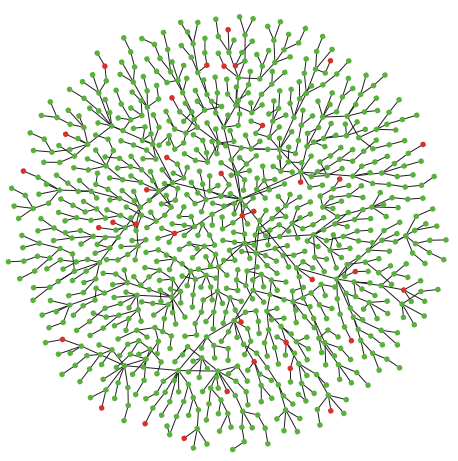
\includegraphics[scale=.65, keepaspectratio]{network_w_Netlogo_2}
			\caption{Esempio di rete generata col programma su NetLogo dopo aver impostato "num-nodes" $= 1000 $, "preferential-attachment $= 0.00 $ e "infected-fraction" $= 0.031 $.}
			\label{fig:NetLogo1}
		\end{center}
\end{figure}
%Ricordiamo, a questo proposito, di aver sostituito alla probabilità di infezione netta $ \tau $ il prodotto $ \tau \cdot exp(-J \tfrac{s}{k}) $, dove con $ \tfrac{s}{k} $ si è indicato la frazione $ s $ di infetti su $ k $ vicini; nel codice sviluppato questa quantità è stata resa dalla variabile "alert" 
Gli agenti - che su NetLogo vengono indicati con il nome di \emph{turtles} - possono essere descritti in termini di tre variabili:
\begin{enumerate}
\item \textit{"state"}, alla quale viene assegnato un valore numerico $ \geq 0 $ sulla base della condizione di salute e che, pertanto, funge da contatore per la durata del periodo d'infezione;
\item \textit{"infected?"}, che può assumere valore vero/falso;
\item \textit{"alert"}, che tiene conto della quantità di vicini infetti (quella che, nel precedente capitolo, veniva indicata come $ \tfrac{s}{k}$).
\end{enumerate}
Come viene reso evidente in \cref{fig:NetLogo1}, i nodi di colore rosso sono quelli infetti; il loro numero viene stabilito a seguito dell'estrazione di un numero casuale fra $ 0 $ e $ 1 $ e del confronto di questo con la quantità "initial-infected". La probabilità che contagino i vertici ai quali sono collegati è anch'essa aleatoria:
\begin{center}
	\begin{lstlisting}[autogobble,language={NetLogo},caption={Porzione di codice in cui si mette in luce il meccanismo di infezione.},label={list:infection_prob}]
		ask turtles with [state > 0] [
    		ask out-link-neighbors with [state = 0] [
      			if random-float 1 < infectivity * exp(-1 * risk-perception * alert) [
        				set state num-states
        				set infected? true
      			]
    		]
  		]  
	\end{lstlisting}
\end{center}
%\begin{center}
%\begin{lstlisting}[language={NetLogo},caption={Porzione di codice in cui si mette in luce il meccanismo di infezione.},label={list:infection_prob}]
%		ask turtles with [state > 0] 
%    		ask out-link-neighbors with [state = 0] 
%      			if random-float 1 < infectivity * exp(-1 * risk-perception * alert) 
%        				set state num-states
%        				set infected? true]]]
%\end{lstlisting}
%\end{center}
Si rimanda all'appendice \ref{appendix:code} per il codice sviluppato per intero.
\section{Analisi sperimentale}
Abbiamo deciso di eseguire una serie di simulazioni sia per una rete poissoniana che per una scale-free. In entrambe le casistiche, abbiamo mantenuto fissati tutti i parametri in gioco meno "perception-risk", che, invece, abbiamo fatto variare da $ 0.10 $ a $ 0.35 $ a passi di $ 0.05 $; abbiamo poi stabilito di ripetere ogni operazione $ 10 $ volte. I valori comuni che abbiamo impostato sono i seguenti:
\begin{itemize}
\item numero di nodi ("num-noded") $ = 1000 $;
\item tasso di infettività ("infectivity") $ = 0.2 $;
\item numero iniziale di infetti ("initial-infected") $ = 0.031 $;
\item durata dell'infezione ("num-states").
\end{itemize}
%\subsection{Caso I: rete poissoniana}
%Abbiamo messo lo slider "preferential-attachment" a $ 0.00 $ ed abbiamo avviato BehaviorSpace; abbiamo atteso che portasse a compimento tutte le esecuzioni
%
%\subsection{Caso II: rete scale-free}
%Per questo scenario, abbiamo impostato lo slider "preferential-attachment" su $ 0.60 $.
L'unica differenza, per quanto riguarda gli slider gestibili dall'utente, sta nel fatto che nel primo caso abbiamo messo "preferential-attachment" pari a $ 0.00 $  - così che la rete generata fosse totalmente aleatoria - mentre nel secondo l'abbiamo posto pari a $ 0.60 $ (si noti la diversa disposizione dei link in \cref{fig:NetLogo2}).
\begin{figure}[t]
		\begin{center}
			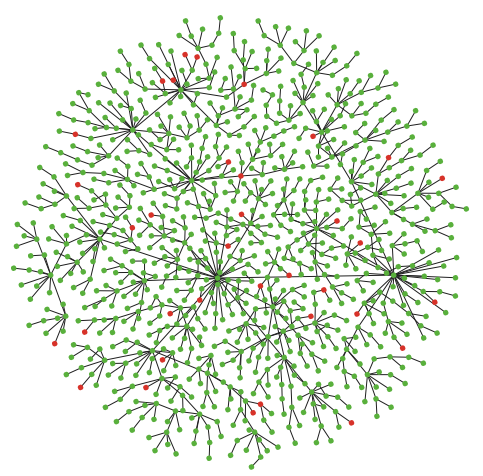
\includegraphics[scale=.65, keepaspectratio]{network_w_Netlogo_3b}
			\caption{Esempio di rete generata col programma su NetLogo dopo aver impostato "num-nodes" $= 1000 $, "preferential-attachment $= 0.60 $ e "infected-fraction" $= 0.031 $.}
			\label{fig:NetLogo2}
		\end{center}
\end{figure}
\\Ad ogni lancio del programma, viene decrementata di un'unità la variabile "state", che, per un individuo infetto, ha valore iniziale pari a "num-states"; quando "state" torna uguale a $ 0 $, si assume che il soggetto sia guarito e il nodo che lo va a rappresentare passa dal rosso al giallo \footnote{Nonostante tornino a fare parte del gruppo dei suscettibili (dal momento che stiamo considerando un modello SIS), preferiamo non colorare di verde gli agenti che si sono ristabiliti dalla malattia per poterli distinguere da quelli che non l'hanno mai contratta.}. Inoltre, ogni agente suscettibile conta il numero di vicini - cioè di nodi che ad esso sono collegati - infetti e imposta questo valore come "alert"; viene poi messo in atto il processo di infezione come mostrato nella porzione di codice \ref{list:infection_prob}. \\Poiché siamo interessati, come già sottolineato, alla frazione di soggetti che non si sono mai ammalati, ne prendiamo nota con la procedura 
\begin{center}
	\begin{lstlisting}[autogobble,language={NetLogo},caption={Metodo che riporta la frazione di suscettibili che non hanno mai contratto l'infezione.},label={list:count_susceptibles}]
		to-report fraction-susceptibles
  			report count turtles with [infected? = false] / count turtles
		end	
	\end{lstlisting}
\end{center}
che viene successivamente sfruttata da BehaviorSpace per stampare il dato ricercato su di un file CSV. \\ Questa operazione viene ripetuta ad ogni "tick", cioè ad ogni istante di tempo; dal momento che è capitato che, nel corso di alcuni test del codice, l'esecuzione non si arrestasse mai, abbiamo aggiunto due stop ad hoc: il primo nel caso in cui si riesca ad estirpare l'epidemia e quindi non ci siano più agenti infetti, il secondo qualora le precauzioni prese non siano sufficienti e la malattia raggiunga tutti gli individui facenti parte della rete.\\Riportiamo di seguito i risultati delle nostre simulazioni.
%\begin{figure*}
%	\begin{minipage}{0.48\textwidth}
%		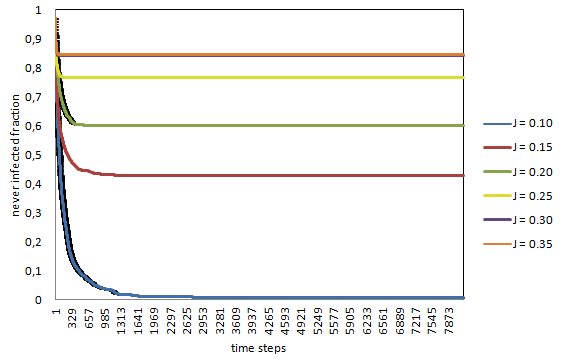
\includegraphics[scale = 0.3]{poisson_errorbars_I}
%		\caption{Andamento della frazione dei suscettibili, nel caso di una rete poissoniana, in funzione di una diversa percezione del rischio.}
%	\end{minipage}
%\hfill
%	\begin{minipage}{0.48\textwidth}
%		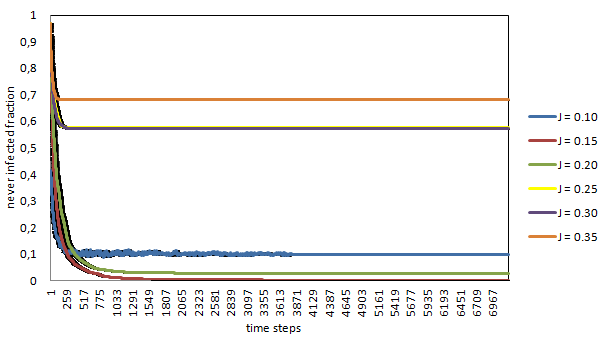
\includegraphics[scale = 0.3]{scalefree_errorbars_I}
%	\caption{Andamento della frazione dei suscettibili, nel caso di una rete scale-free, in funzione di una diversa percezione del rischio.}
%	\end{minipage}
%\end{figure*}
\begin{figure}[h]
		\begin{center}
			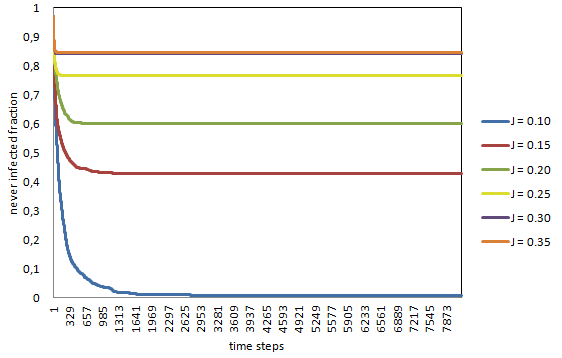
\includegraphics[scale=.7, keepaspectratio]{poisson_I}
			\caption{Andamento della frazione dei suscettibili, nel caso di una rete poissoniana, in funzione di una diversa percezione del rischio.}
			\label{fig:sim_poisson}
		\end{center}
\end{figure}

\begin{figure}
		\begin{center}
			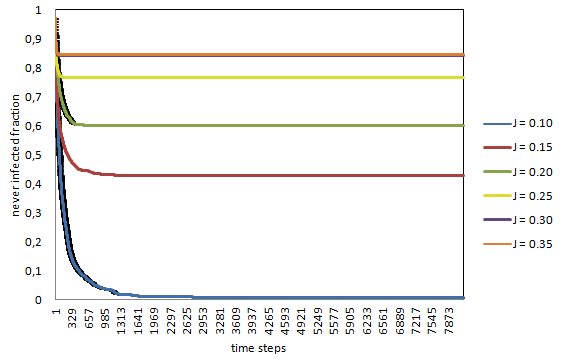
\includegraphics[scale=.7, keepaspectratio]{poisson_errorbars_I}
			\caption{Come in \cref{fig:sim_poisson} ma con barre d'errore.}
			\label{fig:sim_poisson2}
		\end{center}
\end{figure}

\begin{figure}
		\begin{center}
			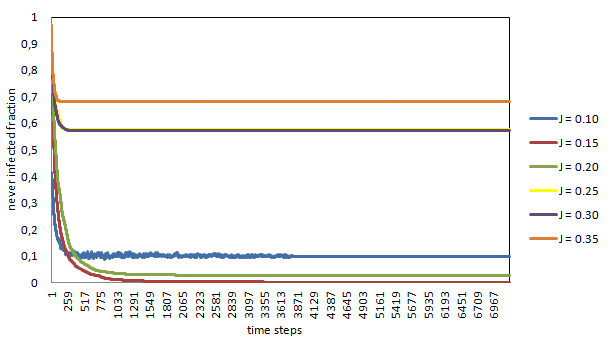
\includegraphics[scale=.7, keepaspectratio]{scalefree_I}
			\caption{Andamento della frazione dei suscettibili, nel caso di una rete scale-free, in funzione di una diversa percezione del rischio.}
			\label{fig:sim_scalefree}
		\end{center}
\end{figure}	

\begin{figure}
		\begin{center}
			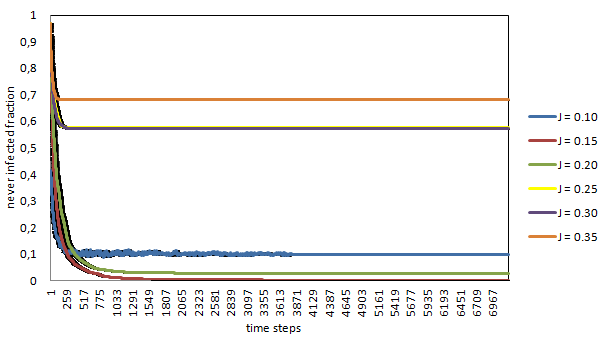
\includegraphics[scale=.7, keepaspectratio]{scalefree_errorbars_I}
			\caption{Come in \cref{fig:sim_scalefree} ma con barre d'errore.}
			\label{fig:sim_scalefree2}
		\end{center}
\end{figure}	